\documentclass[a4paper]{book}
\usepackage{makeidx}
\usepackage{natbib}
\usepackage{graphicx}
\usepackage{multicol}
\usepackage{float}
\usepackage{listings}
\usepackage{color}
\usepackage{ifthen}
\usepackage[table]{xcolor}
\usepackage{textcomp}
\usepackage{alltt}
\usepackage{ifpdf}
\ifpdf
\usepackage[pdftex,
            pagebackref=true,
            colorlinks=true,
            linkcolor=blue,
            unicode
           ]{hyperref}
\else
\usepackage[ps2pdf,
            pagebackref=true,
            colorlinks=true,
            linkcolor=blue,
            unicode
           ]{hyperref}
\usepackage{pspicture}
\fi
\usepackage[utf8]{inputenc}
\usepackage{mathptmx}
\usepackage[scaled=.90]{helvet}
\usepackage{courier}
\usepackage{sectsty}
\usepackage[titles]{tocloft}
\usepackage{doxygen}
\lstset{language=C++,inputencoding=utf8,basicstyle=\footnotesize,breaklines=true,breakatwhitespace=true,tabsize=8,numbers=left }
\makeindex
\setcounter{tocdepth}{3}
\renewcommand{\footrulewidth}{0.4pt}
\renewcommand{\familydefault}{\sfdefault}
\hfuzz=15pt
\setlength{\emergencystretch}{15pt}
\hbadness=750
\tolerance=750
\begin{document}
\hypersetup{pageanchor=false,citecolor=blue}
\begin{titlepage}
\vspace*{7cm}
\begin{center}
{\Large \-Occluded \-Geometry \-Estimation \\[1ex]\large 1.\-0 }\\
\vspace*{1cm}
{\large \-Generated by Doxygen 1.7.6.1}\\
\vspace*{0.5cm}
{\small Tue Jul 30 2013 23:02:21}\\
\end{center}
\end{titlepage}
\clearemptydoublepage
\pagenumbering{roman}
\tableofcontents
\clearemptydoublepage
\pagenumbering{arabic}
\hypersetup{pageanchor=true,citecolor=blue}
\chapter{\-Class \-Index}
\section{\-Class \-List}
\-Here are the classes, structs, unions and interfaces with brief descriptions\-:\begin{DoxyCompactList}
\item\contentsline{section}{\hyperlink{class_helper_functions}{\-Helper\-Functions} \\*\-This class is a grouping of functions that can be accessed from any }{\pageref{class_helper_functions}}{}
\item\contentsline{section}{\hyperlink{class_my_point_representation}{\-My\-Point\-Representation} }{\pageref{class_my_point_representation}}{}
\item\contentsline{section}{\hyperlink{classobject__reconstruction__node}{object\-\_\-reconstruction\-\_\-node} }{\pageref{classobject__reconstruction__node}}{}
\item\contentsline{section}{\hyperlink{class_object_candidate_extractor}{\-Object\-Candidate\-Extractor} }{\pageref{class_object_candidate_extractor}}{}
\item\contentsline{section}{\hyperlink{class_point_cloud_accumulator}{\-Point\-Cloud\-Accumulator} \\*\-This class takes two point clouds and merges them together }{\pageref{class_point_cloud_accumulator}}{}
\end{DoxyCompactList}

\chapter{\-File \-Index}
\section{\-File \-List}
\-Here is a list of all files with brief descriptions\-:\begin{DoxyCompactList}
\item\contentsline{section}{ros/include/\hyperlink{_helper_functions_8h}{\-Helper\-Functions.\-h} }{\pageref{_helper_functions_8h}}{}
\item\contentsline{section}{ros/include/\hyperlink{_object_candidate_extractor_8h}{\-Object\-Candidate\-Extractor.\-h} }{\pageref{_object_candidate_extractor_8h}}{}
\item\contentsline{section}{ros/include/\hyperlink{_occlusion_repair_8h}{\-Occlusion\-Repair.\-h} }{\pageref{_occlusion_repair_8h}}{}
\item\contentsline{section}{ros/include/\hyperlink{_point_cloud_accumulator_8h}{\-Point\-Cloud\-Accumulator.\-h} }{\pageref{_point_cloud_accumulator_8h}}{}
\item\contentsline{section}{ros/nodes/\hyperlink{object__reconstruction_8cpp}{object\-\_\-reconstruction.\-cpp} }{\pageref{object__reconstruction_8cpp}}{}
\item\contentsline{section}{ros/src/\hyperlink{_helper_functions_8cpp}{\-Helper\-Functions.\-cpp} }{\pageref{_helper_functions_8cpp}}{}
\item\contentsline{section}{ros/src/\hyperlink{_object_candidate_extractor_8cpp}{\-Object\-Candidate\-Extractor.\-cpp} }{\pageref{_object_candidate_extractor_8cpp}}{}
\item\contentsline{section}{ros/src/\hyperlink{_occlusion_repair_8cpp}{\-Occlusion\-Repair.\-cpp} }{\pageref{_occlusion_repair_8cpp}}{}
\item\contentsline{section}{ros/src/\hyperlink{_point_cloud_accumulator_8cpp}{\-Point\-Cloud\-Accumulator.\-cpp} }{\pageref{_point_cloud_accumulator_8cpp}}{}
\end{DoxyCompactList}

\chapter{\-Class \-Documentation}
\hypertarget{class_helper_functions}{\section{\-Helper\-Functions \-Class \-Reference}
\label{class_helper_functions}\index{\-Helper\-Functions@{\-Helper\-Functions}}
}


\-This class is a grouping of functions that can be accessed from any.  


\subsection*{\-Static \-Public \-Member \-Functions}
\begin{DoxyCompactItemize}
\item 
static \hyperlink{_helper_functions_8h_abb956d1047f4dd2c956fe3cb0dd0004d}{\-Point\-Cloud} \hyperlink{class_helper_functions_a2e817646b20092d5f7179ba89635b50f}{\-Prepare\-Point\-Cloud} (\hyperlink{_helper_functions_8h_abb956d1047f4dd2c956fe3cb0dd0004d}{\-Point\-Cloud} input\-\_\-cloud)
\begin{DoxyCompactList}\small\item\em \-This function is responsible for pre-\/processing the input pointcloud before we attempt object reconstruction. \end{DoxyCompactList}\item 
static bool \hyperlink{class_helper_functions_a4b25abbfbd620e9218b2949c758a8872}{\-Write\-To\-P\-C\-D} (std\-::string file\-\_\-name, \hyperlink{_helper_functions_8h_abb956d1047f4dd2c956fe3cb0dd0004d}{\-Point\-Cloud} input\-\_\-cloud)
\begin{DoxyCompactList}\small\item\em \-A function that is used to write a standard \-P\-C\-L pointcloud to a \-Point\-Cloud \-Data \-File (\-P\-C\-D). \end{DoxyCompactList}\item 
static bool \hyperlink{class_helper_functions_a4428222439104c10e58e04958a231c37}{\-Write\-Multiple\-To\-P\-C\-D} (std\-::string file\-\_\-name, std\-::vector$<$ \hyperlink{_helper_functions_8h_abb956d1047f4dd2c956fe3cb0dd0004d}{\-Point\-Cloud} $>$ input\-\_\-clouds)
\begin{DoxyCompactList}\small\item\em \-Function that is used to write out multiple \-Point\-Clouds to \-Multiple \-P\-C\-D \-Files. \end{DoxyCompactList}\item 
static \hyperlink{_helper_functions_8h_a1ee4898d5040989c5fad6726ea5b2056}{\-P\-C\-L\-Mesh} \hyperlink{class_helper_functions_a51d22836259590b5e4e27c551bba93f3}{\-Convert\-Cloud\-To\-Mesh} (std\-::string file\-\_\-name, \hyperlink{_helper_functions_8h_abb956d1047f4dd2c956fe3cb0dd0004d}{\-Point\-Cloud} input\-\_\-cloud)
\item 
static bool \hyperlink{class_helper_functions_a5b355421138212e50b90b120734854ef}{\-Publish\-Mesh\-Marker} (ros\-::\-Publisher mesh\-\_\-publisher, std\-::string file\-\_\-name)
\end{DoxyCompactItemize}


\subsection{\-Detailed \-Description}
\-This class is a grouping of functions that can be accessed from any. 

\subsection{\-Member \-Function \-Documentation}
\hypertarget{class_helper_functions_a51d22836259590b5e4e27c551bba93f3}{\index{\-Helper\-Functions@{\-Helper\-Functions}!\-Convert\-Cloud\-To\-Mesh@{\-Convert\-Cloud\-To\-Mesh}}
\index{\-Convert\-Cloud\-To\-Mesh@{\-Convert\-Cloud\-To\-Mesh}!HelperFunctions@{\-Helper\-Functions}}
\subsubsection[{\-Convert\-Cloud\-To\-Mesh}]{\setlength{\rightskip}{0pt plus 5cm}{\bf \-P\-C\-L\-Mesh} {\bf \-Helper\-Functions\-::\-Convert\-Cloud\-To\-Mesh} (
\begin{DoxyParamCaption}
\item[{std\-::string}]{file\-\_\-name, }
\item[{{\bf \-Point\-Cloud}}]{input\-\_\-cloud}
\end{DoxyParamCaption}
)\hspace{0.3cm}{\ttfamily  \mbox{[}static\mbox{]}}}}\label{class_helper_functions_a51d22836259590b5e4e27c551bba93f3}
\hypertarget{class_helper_functions_a2e817646b20092d5f7179ba89635b50f}{\index{\-Helper\-Functions@{\-Helper\-Functions}!\-Prepare\-Point\-Cloud@{\-Prepare\-Point\-Cloud}}
\index{\-Prepare\-Point\-Cloud@{\-Prepare\-Point\-Cloud}!HelperFunctions@{\-Helper\-Functions}}
\subsubsection[{\-Prepare\-Point\-Cloud}]{\setlength{\rightskip}{0pt plus 5cm}{\bf \-Point\-Cloud} {\bf \-Helper\-Functions\-::\-Prepare\-Point\-Cloud} (
\begin{DoxyParamCaption}
\item[{{\bf \-Point\-Cloud}}]{input\-\_\-cloud}
\end{DoxyParamCaption}
)\hspace{0.3cm}{\ttfamily  \mbox{[}static\mbox{]}}}}\label{class_helper_functions_a2e817646b20092d5f7179ba89635b50f}


\-This function is responsible for pre-\/processing the input pointcloud before we attempt object reconstruction. 

\-It will perform both a statistical outlier removal which will take the current point cloud and remove any points that are to far removed from all of its neighbors (cleaning up noise). \-It will also perform subsamling in order to make the following computations more efficient.


\begin{DoxyParams}{\-Parameters}
{\em input\-\_\-cloud} & \-The point cloud which we want to perform the pre-\/processing on.\\
\hline
\end{DoxyParams}
\begin{DoxyReturn}{\-Returns}
\-A pre-\/processed (noise removed \& subsampled) pointcloud. 
\end{DoxyReturn}
\hypertarget{class_helper_functions_a5b355421138212e50b90b120734854ef}{\index{\-Helper\-Functions@{\-Helper\-Functions}!\-Publish\-Mesh\-Marker@{\-Publish\-Mesh\-Marker}}
\index{\-Publish\-Mesh\-Marker@{\-Publish\-Mesh\-Marker}!HelperFunctions@{\-Helper\-Functions}}
\subsubsection[{\-Publish\-Mesh\-Marker}]{\setlength{\rightskip}{0pt plus 5cm}bool {\bf \-Helper\-Functions\-::\-Publish\-Mesh\-Marker} (
\begin{DoxyParamCaption}
\item[{ros\-::\-Publisher}]{mesh\-\_\-publisher, }
\item[{std\-::string}]{file\-\_\-name}
\end{DoxyParamCaption}
)\hspace{0.3cm}{\ttfamily  \mbox{[}static\mbox{]}}}}\label{class_helper_functions_a5b355421138212e50b90b120734854ef}
\hypertarget{class_helper_functions_a4428222439104c10e58e04958a231c37}{\index{\-Helper\-Functions@{\-Helper\-Functions}!\-Write\-Multiple\-To\-P\-C\-D@{\-Write\-Multiple\-To\-P\-C\-D}}
\index{\-Write\-Multiple\-To\-P\-C\-D@{\-Write\-Multiple\-To\-P\-C\-D}!HelperFunctions@{\-Helper\-Functions}}
\subsubsection[{\-Write\-Multiple\-To\-P\-C\-D}]{\setlength{\rightskip}{0pt plus 5cm}bool {\bf \-Helper\-Functions\-::\-Write\-Multiple\-To\-P\-C\-D} (
\begin{DoxyParamCaption}
\item[{std\-::string}]{file\-\_\-name, }
\item[{std\-::vector$<$ {\bf \-Point\-Cloud} $>$}]{input\-\_\-clouds}
\end{DoxyParamCaption}
)\hspace{0.3cm}{\ttfamily  \mbox{[}static\mbox{]}}}}\label{class_helper_functions_a4428222439104c10e58e04958a231c37}


\-Function that is used to write out multiple \-Point\-Clouds to \-Multiple \-P\-C\-D \-Files. 


\begin{DoxyParams}{\-Parameters}
{\em file\-\_\-name} & \-Desired series of file names. \-Index will be appended to it. \\
\hline
{\em input\-\_\-clouds} & \-A std\-::vector that contains at least 2 \-P\-C\-L \-Point\-Cloud. \\
\hline
\end{DoxyParams}
\begin{DoxyReturn}{\-Returns}
\-If we where able to properly write to \-P\-C\-D files. 
\end{DoxyReturn}
\hypertarget{class_helper_functions_a4b25abbfbd620e9218b2949c758a8872}{\index{\-Helper\-Functions@{\-Helper\-Functions}!\-Write\-To\-P\-C\-D@{\-Write\-To\-P\-C\-D}}
\index{\-Write\-To\-P\-C\-D@{\-Write\-To\-P\-C\-D}!HelperFunctions@{\-Helper\-Functions}}
\subsubsection[{\-Write\-To\-P\-C\-D}]{\setlength{\rightskip}{0pt plus 5cm}bool {\bf \-Helper\-Functions\-::\-Write\-To\-P\-C\-D} (
\begin{DoxyParamCaption}
\item[{std\-::string}]{file\-\_\-name, }
\item[{{\bf \-Point\-Cloud}}]{input\-\_\-cloud}
\end{DoxyParamCaption}
)\hspace{0.3cm}{\ttfamily  \mbox{[}static\mbox{]}}}}\label{class_helper_functions_a4b25abbfbd620e9218b2949c758a8872}


\-A function that is used to write a standard \-P\-C\-L pointcloud to a \-Point\-Cloud \-Data \-File (\-P\-C\-D). 


\begin{DoxyParams}{\-Parameters}
{\em file\-\_\-name} & \-The file name as a string that you want the \-P\-C\-D file to have. \\
\hline
{\em input\-\_\-cloud} & \-The \-P\-C\-L pointcloud that you want to save into an \-A\-S\-C\-I\-I \-P\-C\-D file.\\
\hline
\end{DoxyParams}
\begin{DoxyReturn}{\-Returns}
\-If we where able to verify if the point cloud was saved to the file properly or not. 
\end{DoxyReturn}


\-The documentation for this class was generated from the following files\-:\begin{DoxyCompactItemize}
\item 
ros/include/\hyperlink{_helper_functions_8h}{\-Helper\-Functions.\-h}\item 
ros/src/\hyperlink{_helper_functions_8cpp}{\-Helper\-Functions.\-cpp}\end{DoxyCompactItemize}

\hypertarget{class_my_point_representation}{\section{\-My\-Point\-Representation \-Class \-Reference}
\label{class_my_point_representation}\index{\-My\-Point\-Representation@{\-My\-Point\-Representation}}
}
\subsection*{\-Public \-Member \-Functions}
\begin{DoxyCompactItemize}
\item 
\hypertarget{class_my_point_representation_adaf372e3a1093398b90a3216494e8a1d}{virtual void {\bfseries copy\-To\-Float\-Array} (const \hyperlink{_helper_functions_8hpp_af8717e40603e7d4bcd56c56ec09aa10e}{\-Point\-Normal\-T} \&p, float $\ast$out) const }\label{class_my_point_representation_adaf372e3a1093398b90a3216494e8a1d}

\end{DoxyCompactItemize}


\-The documentation for this class was generated from the following file\-:\begin{DoxyCompactItemize}
\item 
ros/include/\-Point\-Cloud\-Accumulator.\-h\end{DoxyCompactItemize}

\hypertarget{classobject__reconstruction__node}{\section{object\-\_\-reconstruction\-\_\-node \-Class \-Reference}
\label{classobject__reconstruction__node}\index{object\-\_\-reconstruction\-\_\-node@{object\-\_\-reconstruction\-\_\-node}}
}


\-This class is responisble for handeling everything that is related to the object reconstruction.  


\subsection*{\-Public \-Member \-Functions}
\begin{DoxyCompactItemize}
\item 
\hyperlink{classobject__reconstruction__node_a6e45abbc296968691a0195ebcdf11fd0}{object\-\_\-reconstruction\-\_\-node} ()
\begin{DoxyCompactList}\small\item\em \-Constructor method for the \-Object\-Reconstruction\-Node. \end{DoxyCompactList}\end{DoxyCompactItemize}


\subsection{\-Detailed \-Description}
\-This class is responisble for handeling everything that is related to the object reconstruction. 

\-It is the public interface for all of the backend processing that is required. \-It advertises the following services that the user are able to call\-: 
\begin{DoxyItemize}
\item \-Fix\-Occlusions
\end{DoxyItemize}

\subsection{\-Constructor \& \-Destructor \-Documentation}
\hypertarget{classobject__reconstruction__node_a6e45abbc296968691a0195ebcdf11fd0}{\index{object\-\_\-reconstruction\-\_\-node@{object\-\_\-reconstruction\-\_\-node}!object\-\_\-reconstruction\-\_\-node@{object\-\_\-reconstruction\-\_\-node}}
\index{object\-\_\-reconstruction\-\_\-node@{object\-\_\-reconstruction\-\_\-node}!object_reconstruction_node@{object\-\_\-reconstruction\-\_\-node}}
\subsubsection[{object\-\_\-reconstruction\-\_\-node}]{\setlength{\rightskip}{0pt plus 5cm}{\bf object\-\_\-reconstruction\-\_\-node\-::object\-\_\-reconstruction\-\_\-node} (
\begin{DoxyParamCaption}
{}
\end{DoxyParamCaption}
)\hspace{0.3cm}{\ttfamily  \mbox{[}inline\mbox{]}}}}\label{classobject__reconstruction__node_a6e45abbc296968691a0195ebcdf11fd0}


\-Constructor method for the \-Object\-Reconstruction\-Node. 

\-This method creates all of the required connections for this \-R\-O\-S node as well as starting all of the subcomponents that this functionality requires. 

\-The documentation for this class was generated from the following file\-:\begin{DoxyCompactItemize}
\item 
ros/nodes/\hyperlink{object__reconstruction_8cpp}{object\-\_\-reconstruction.\-cpp}\end{DoxyCompactItemize}

\hypertarget{class_object_candidate_extractor}{\section{\-Object\-Candidate\-Extractor \-Class \-Reference}
\label{class_object_candidate_extractor}\index{\-Object\-Candidate\-Extractor@{\-Object\-Candidate\-Extractor}}
}


\-This class is responsible for finding groups of points in a point cloud which could represent real world objects.  


\subsection*{\-Public \-Member \-Functions}
\begin{DoxyCompactItemize}
\item 
\hyperlink{class_object_candidate_extractor_a41916df0d27e926a337fff6e7e762010}{\-Object\-Candidate\-Extractor} ()
\begin{DoxyCompactList}\small\item\em \-Responsible for initializing and setting up all resources that are required to perform object candidate extraction. \end{DoxyCompactList}\item 
virtual \hyperlink{class_object_candidate_extractor_ad1aa824172a7d2e6002d5d7e3104d5d3}{$\sim$\-Object\-Candidate\-Extractor} ()
\begin{DoxyCompactList}\small\item\em \-Standard destructor that is used to free up any memory or \-R\-O\-S connections that where created. \end{DoxyCompactList}\item 
std\-::vector$<$ \hyperlink{_helper_functions_8h_abb956d1047f4dd2c956fe3cb0dd0004d}{\-Point\-Cloud} $>$ \hyperlink{class_object_candidate_extractor_a6a4adbcec19f94bc6073a4b2c2fa6f66}{\-Extract\-Candidate\-Objects} (\hyperlink{_helper_functions_8h_abb956d1047f4dd2c956fe3cb0dd0004d}{\-Point\-Cloud} input\-\_\-cloud)
\begin{DoxyCompactList}\small\item\em \-This function takes in a \-P\-C\-L \-Point \-Cloud and finds any candidate objects contained in the scene. \end{DoxyCompactList}\item 
\hyperlink{_helper_functions_8h_abb956d1047f4dd2c956fe3cb0dd0004d}{\-Point\-Cloud} \hyperlink{class_object_candidate_extractor_a6d54ffc5a2c1690b418107a31e34dfd2}{\-Restore\-Plane\-Interaction} (pcl\-::\-Model\-Coefficients\-::\-Ptr i\-\_\-coefficients, \hyperlink{_helper_functions_8h_abb956d1047f4dd2c956fe3cb0dd0004d}{\-Point\-Cloud} i\-\_\-model)
\item 
bool \hyperlink{class_object_candidate_extractor_ab8848f6d86f7d7798ea30c2e04ae8b59}{\-Publish\-Object\-Candidates} (std\-::vector$<$ \hyperlink{_helper_functions_8h_abb956d1047f4dd2c956fe3cb0dd0004d}{\-Point\-Cloud} $>$ input\-\_\-vector)
\begin{DoxyCompactList}\small\item\em \-Function that takes in multiple object candidate point clouds and creates a single ros message for them. \end{DoxyCompactList}\end{DoxyCompactItemize}
\subsection*{\-Protected \-Attributes}
\begin{DoxyCompactItemize}
\item 
ros\-::\-Node\-Handle \hyperlink{class_object_candidate_extractor_a9a0da45687232f96360f76175a3cb097}{m\-\_\-node\-\_\-handler}
\begin{DoxyCompactList}\small\item\em \-Node \-Handler for the \hyperlink{class_object_candidate_extractor}{\-Object\-Candidate\-Extractor} class. \end{DoxyCompactList}\item 
ros\-::\-Publisher \hyperlink{class_object_candidate_extractor_a3b5cd0451266eafe0aba2d950a7434e8}{m\-\_\-object\-\_\-candidates\-\_\-publisher}
\begin{DoxyCompactList}\small\item\em \-A \-R\-O\-S publisher for the compiled object candidates. \end{DoxyCompactList}\end{DoxyCompactItemize}


\subsection{\-Detailed \-Description}
\-This class is responsible for finding groups of points in a point cloud which could represent real world objects. 

\begin{DoxyAuthor}{\-Author}
\-Matthew \-S \-Roscoe 
\end{DoxyAuthor}
\begin{DoxyDate}{\-Date}
\-July 30th 2013 
\end{DoxyDate}
\begin{DoxyCopyright}{\-Copyright}
\-G\-N\-U \-Public \-License. 
\end{DoxyCopyright}


\subsection{\-Constructor \& \-Destructor \-Documentation}
\hypertarget{class_object_candidate_extractor_a41916df0d27e926a337fff6e7e762010}{\index{\-Object\-Candidate\-Extractor@{\-Object\-Candidate\-Extractor}!\-Object\-Candidate\-Extractor@{\-Object\-Candidate\-Extractor}}
\index{\-Object\-Candidate\-Extractor@{\-Object\-Candidate\-Extractor}!ObjectCandidateExtractor@{\-Object\-Candidate\-Extractor}}
\subsubsection[{\-Object\-Candidate\-Extractor}]{\setlength{\rightskip}{0pt plus 5cm}{\bf \-Object\-Candidate\-Extractor\-::\-Object\-Candidate\-Extractor} (
\begin{DoxyParamCaption}
{}
\end{DoxyParamCaption}
)}}\label{class_object_candidate_extractor_a41916df0d27e926a337fff6e7e762010}


\-Responsible for initializing and setting up all resources that are required to perform object candidate extraction. 

\hypertarget{class_object_candidate_extractor_ad1aa824172a7d2e6002d5d7e3104d5d3}{\index{\-Object\-Candidate\-Extractor@{\-Object\-Candidate\-Extractor}!$\sim$\-Object\-Candidate\-Extractor@{$\sim$\-Object\-Candidate\-Extractor}}
\index{$\sim$\-Object\-Candidate\-Extractor@{$\sim$\-Object\-Candidate\-Extractor}!ObjectCandidateExtractor@{\-Object\-Candidate\-Extractor}}
\subsubsection[{$\sim$\-Object\-Candidate\-Extractor}]{\setlength{\rightskip}{0pt plus 5cm}{\bf \-Object\-Candidate\-Extractor\-::$\sim$\-Object\-Candidate\-Extractor} (
\begin{DoxyParamCaption}
{}
\end{DoxyParamCaption}
)\hspace{0.3cm}{\ttfamily  \mbox{[}virtual\mbox{]}}}}\label{class_object_candidate_extractor_ad1aa824172a7d2e6002d5d7e3104d5d3}


\-Standard destructor that is used to free up any memory or \-R\-O\-S connections that where created. 



\subsection{\-Member \-Function \-Documentation}
\hypertarget{class_object_candidate_extractor_a6a4adbcec19f94bc6073a4b2c2fa6f66}{\index{\-Object\-Candidate\-Extractor@{\-Object\-Candidate\-Extractor}!\-Extract\-Candidate\-Objects@{\-Extract\-Candidate\-Objects}}
\index{\-Extract\-Candidate\-Objects@{\-Extract\-Candidate\-Objects}!ObjectCandidateExtractor@{\-Object\-Candidate\-Extractor}}
\subsubsection[{\-Extract\-Candidate\-Objects}]{\setlength{\rightskip}{0pt plus 5cm}std\-::vector$<$ {\bf \-Point\-Cloud} $>$ {\bf \-Object\-Candidate\-Extractor\-::\-Extract\-Candidate\-Objects} (
\begin{DoxyParamCaption}
\item[{{\bf \-Point\-Cloud}}]{input\-\_\-cloud}
\end{DoxyParamCaption}
)}}\label{class_object_candidate_extractor_a6a4adbcec19f94bc6073a4b2c2fa6f66}


\-This function takes in a \-P\-C\-L \-Point \-Cloud and finds any candidate objects contained in the scene. 


\begin{DoxyParams}{\-Parameters}
{\em input\-\_\-cloud} & \-The \-P\-C\-L \-Point\-Cloud that will be checked for candidate objects. \\
\hline
\end{DoxyParams}
\begin{DoxyReturn}{\-Returns}
\-A \-Vector which contains all of the candidate objects. 
\end{DoxyReturn}
\hypertarget{class_object_candidate_extractor_ab8848f6d86f7d7798ea30c2e04ae8b59}{\index{\-Object\-Candidate\-Extractor@{\-Object\-Candidate\-Extractor}!\-Publish\-Object\-Candidates@{\-Publish\-Object\-Candidates}}
\index{\-Publish\-Object\-Candidates@{\-Publish\-Object\-Candidates}!ObjectCandidateExtractor@{\-Object\-Candidate\-Extractor}}
\subsubsection[{\-Publish\-Object\-Candidates}]{\setlength{\rightskip}{0pt plus 5cm}bool {\bf \-Object\-Candidate\-Extractor\-::\-Publish\-Object\-Candidates} (
\begin{DoxyParamCaption}
\item[{std\-::vector$<$ {\bf \-Point\-Cloud} $>$}]{input\-\_\-vector}
\end{DoxyParamCaption}
)}}\label{class_object_candidate_extractor_ab8848f6d86f7d7798ea30c2e04ae8b59}


\-Function that takes in multiple object candidate point clouds and creates a single ros message for them. 

\-This function takes in a \-S\-T\-D \-Vector of \-P\-C\-L \-Point \-Clouds where each cloud is a candidate object. \-It will then combine them all into one single \-S\-T\-D\-\_\-\-M\-S\-G\-S\-::\-Point\-Cloud2 message that can be published through \-R\-O\-S.


\begin{DoxyParams}{\-Parameters}
{\em input\-\_\-vector} & \\
\hline
\end{DoxyParams}
\begin{DoxyReturn}{\-Returns}

\end{DoxyReturn}
\hypertarget{class_object_candidate_extractor_a6d54ffc5a2c1690b418107a31e34dfd2}{\index{\-Object\-Candidate\-Extractor@{\-Object\-Candidate\-Extractor}!\-Restore\-Plane\-Interaction@{\-Restore\-Plane\-Interaction}}
\index{\-Restore\-Plane\-Interaction@{\-Restore\-Plane\-Interaction}!ObjectCandidateExtractor@{\-Object\-Candidate\-Extractor}}
\subsubsection[{\-Restore\-Plane\-Interaction}]{\setlength{\rightskip}{0pt plus 5cm}{\bf \-Point\-Cloud} {\bf \-Object\-Candidate\-Extractor\-::\-Restore\-Plane\-Interaction} (
\begin{DoxyParamCaption}
\item[{pcl\-::\-Model\-Coefficients\-::\-Ptr}]{i\-\_\-coefficients, }
\item[{{\bf \-Point\-Cloud}}]{i\-\_\-model}
\end{DoxyParamCaption}
)}}\label{class_object_candidate_extractor_a6d54ffc5a2c1690b418107a31e34dfd2}


\subsection{\-Member \-Data \-Documentation}
\hypertarget{class_object_candidate_extractor_a9a0da45687232f96360f76175a3cb097}{\index{\-Object\-Candidate\-Extractor@{\-Object\-Candidate\-Extractor}!m\-\_\-node\-\_\-handler@{m\-\_\-node\-\_\-handler}}
\index{m\-\_\-node\-\_\-handler@{m\-\_\-node\-\_\-handler}!ObjectCandidateExtractor@{\-Object\-Candidate\-Extractor}}
\subsubsection[{m\-\_\-node\-\_\-handler}]{\setlength{\rightskip}{0pt plus 5cm}ros\-::\-Node\-Handle {\bf \-Object\-Candidate\-Extractor\-::m\-\_\-node\-\_\-handler}\hspace{0.3cm}{\ttfamily  \mbox{[}protected\mbox{]}}}}\label{class_object_candidate_extractor_a9a0da45687232f96360f76175a3cb097}


\-Node \-Handler for the \hyperlink{class_object_candidate_extractor}{\-Object\-Candidate\-Extractor} class. 

\hypertarget{class_object_candidate_extractor_a3b5cd0451266eafe0aba2d950a7434e8}{\index{\-Object\-Candidate\-Extractor@{\-Object\-Candidate\-Extractor}!m\-\_\-object\-\_\-candidates\-\_\-publisher@{m\-\_\-object\-\_\-candidates\-\_\-publisher}}
\index{m\-\_\-object\-\_\-candidates\-\_\-publisher@{m\-\_\-object\-\_\-candidates\-\_\-publisher}!ObjectCandidateExtractor@{\-Object\-Candidate\-Extractor}}
\subsubsection[{m\-\_\-object\-\_\-candidates\-\_\-publisher}]{\setlength{\rightskip}{0pt plus 5cm}ros\-::\-Publisher {\bf \-Object\-Candidate\-Extractor\-::m\-\_\-object\-\_\-candidates\-\_\-publisher}\hspace{0.3cm}{\ttfamily  \mbox{[}protected\mbox{]}}}}\label{class_object_candidate_extractor_a3b5cd0451266eafe0aba2d950a7434e8}


\-A \-R\-O\-S publisher for the compiled object candidates. 



\-The documentation for this class was generated from the following files\-:\begin{DoxyCompactItemize}
\item 
ros/include/\hyperlink{_object_candidate_extractor_8h}{\-Object\-Candidate\-Extractor.\-h}\item 
ros/src/\hyperlink{_object_candidate_extractor_8cpp}{\-Object\-Candidate\-Extractor.\-cpp}\end{DoxyCompactItemize}

\hypertarget{class_point_cloud_accumulator}{\section{\-Point\-Cloud\-Accumulator \-Class \-Reference}
\label{class_point_cloud_accumulator}\index{\-Point\-Cloud\-Accumulator@{\-Point\-Cloud\-Accumulator}}
}
\subsection*{\-Public \-Member \-Functions}
\begin{DoxyCompactItemize}
\item 
\hypertarget{class_point_cloud_accumulator_a24d93cde9ce3cce292779934f2b97ede}{\-Point\-Cloud {\bfseries \-Accumulate\-Point\-Clouds} (int accumulation\-\_\-time)}\label{class_point_cloud_accumulator_a24d93cde9ce3cce292779934f2b97ede}

\end{DoxyCompactItemize}
\subsection*{\-Protected \-Attributes}
\begin{DoxyCompactItemize}
\item 
\hypertarget{class_point_cloud_accumulator_a6ebb0ca53506f1ae2d0f6e411e2dff66}{int {\bfseries m\-\_\-point\-\_\-cloud\-\_\-count}}\label{class_point_cloud_accumulator_a6ebb0ca53506f1ae2d0f6e411e2dff66}

\item 
\hypertarget{class_point_cloud_accumulator_af8ef35b00c6d547b8d3fa89ad8a8b49a}{std\-::string {\bfseries m\-\_\-frame\-\_\-id}}\label{class_point_cloud_accumulator_af8ef35b00c6d547b8d3fa89ad8a8b49a}

\item 
\hypertarget{class_point_cloud_accumulator_a7ea0dd4449475e6939cefbdb0fd260c5}{\-Eigen\-::\-Matrix4f {\bfseries m\-\_\-global\-\_\-transform}}\label{class_point_cloud_accumulator_a7ea0dd4449475e6939cefbdb0fd260c5}

\item 
\hypertarget{class_point_cloud_accumulator_a0db3c1a8e6de37bcb25c260626d63ff0}{\-Point\-Cloud {\bfseries m\-\_\-accumulated\-\_\-cloud}}\label{class_point_cloud_accumulator_a0db3c1a8e6de37bcb25c260626d63ff0}

\item 
\hypertarget{class_point_cloud_accumulator_ac9070e4cb82ddf04bb50cc2492e597ae}{ros\-::\-Node\-Handle {\bfseries m\-\_\-node\-\_\-handler}}\label{class_point_cloud_accumulator_ac9070e4cb82ddf04bb50cc2492e597ae}

\item 
\hypertarget{class_point_cloud_accumulator_a117cbef73e39daeda50c32212a3cc603}{ros\-::\-Publisher {\bfseries m\-\_\-accumulated\-\_\-point\-\_\-cloud\-\_\-publisher}}\label{class_point_cloud_accumulator_a117cbef73e39daeda50c32212a3cc603}

\end{DoxyCompactItemize}


\-The documentation for this class was generated from the following files\-:\begin{DoxyCompactItemize}
\item 
ros/include/\-Point\-Cloud\-Accumulator.\-h\item 
ros/src/\-Point\-Cloud\-Accumulator.\-cpp\end{DoxyCompactItemize}

\chapter{\-File \-Documentation}
\hypertarget{_helper_functions_8h}{\section{ros/include/\-Helper\-Functions.h \-File \-Reference}
\label{_helper_functions_8h}\index{ros/include/\-Helper\-Functions.\-h@{ros/include/\-Helper\-Functions.\-h}}
}
\-Include dependency graph for \-Helper\-Functions.\-h\-:\nopagebreak
\begin{figure}[H]
\begin{center}
\leavevmode
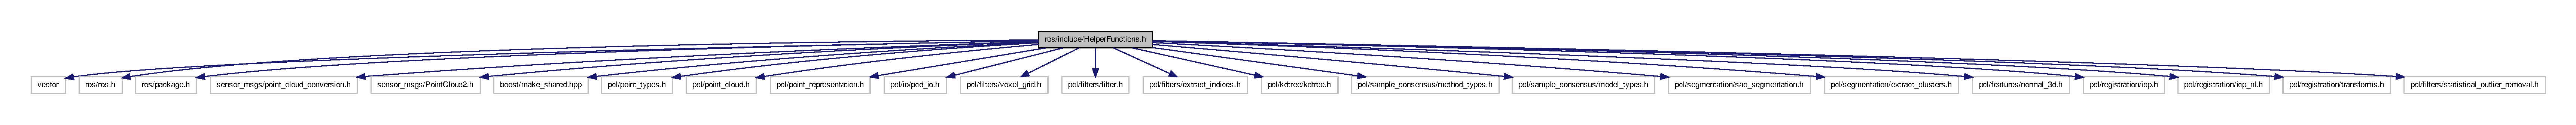
\includegraphics[width=350pt]{_helper_functions_8h__incl}
\end{center}
\end{figure}
\-This graph shows which files directly or indirectly include this file\-:\nopagebreak
\begin{figure}[H]
\begin{center}
\leavevmode
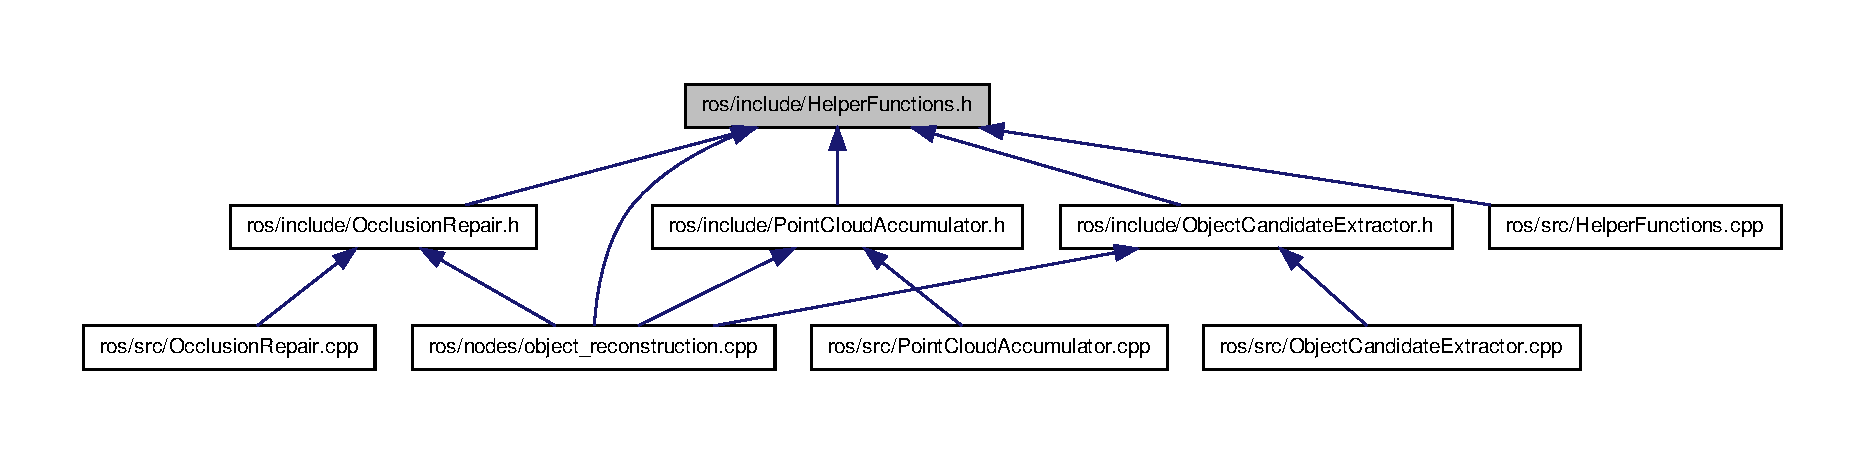
\includegraphics[width=350pt]{_helper_functions_8h__dep__incl}
\end{center}
\end{figure}
\subsection*{\-Classes}
\begin{DoxyCompactItemize}
\item 
class \hyperlink{class_helper_functions}{\-Helper\-Functions}
\begin{DoxyCompactList}\small\item\em \-This class is a grouping of functions that can be accessed from any. \end{DoxyCompactList}\end{DoxyCompactItemize}
\subsection*{\-Typedefs}
\begin{DoxyCompactItemize}
\item 
typedef pcl\-::\-Point\-X\-Y\-Z\-R\-G\-B \hyperlink{_helper_functions_8h_a33eafffb7a0480b3f826230a0ebba532}{\-Point\-T}
\begin{DoxyCompactList}\small\item\em \-Have all points in the project represented by pcl\-::\-Point\-X\-Y\-Z\-R\-G\-B. \end{DoxyCompactList}\item 
typedef \hyperlink{_helper_functions_8h_abb956d1047f4dd2c956fe3cb0dd0004d}{pcl\-::\-Point\-Cloud}$<$ \hyperlink{_helper_functions_8h_a33eafffb7a0480b3f826230a0ebba532}{\-Point\-T} $>$ \hyperlink{_helper_functions_8h_abb956d1047f4dd2c956fe3cb0dd0004d}{\-Point\-Cloud}
\begin{DoxyCompactList}\small\item\em \-Have all pointclouds used in the project made up from \hyperlink{_helper_functions_8h_a33eafffb7a0480b3f826230a0ebba532}{\-Point\-T}. \end{DoxyCompactList}\item 
typedef pcl\-::\-Point\-Normal \hyperlink{_helper_functions_8h_af8717e40603e7d4bcd56c56ec09aa10e}{\-Point\-Normal\-T}
\begin{DoxyCompactList}\small\item\em \-A standard \-P\-C\-L point that also includes \-Normal \-Information for that point. \end{DoxyCompactList}\item 
typedef \hyperlink{_helper_functions_8h_abb956d1047f4dd2c956fe3cb0dd0004d}{pcl\-::\-Point\-Cloud}\*
$<$ \hyperlink{_helper_functions_8h_af8717e40603e7d4bcd56c56ec09aa10e}{\-Point\-Normal\-T} $>$ \hyperlink{_helper_functions_8h_a8bd43f695aeb20e077921614455eaacd}{\-Point\-Cloud\-With\-Normals}
\begin{DoxyCompactList}\small\item\em \-A \-Standard \-P\-C\-L \-Point\-Cloud but where the points all contain normal information as well. \end{DoxyCompactList}\end{DoxyCompactItemize}


\subsection{\-Typedef \-Documentation}
\hypertarget{_helper_functions_8h_abb956d1047f4dd2c956fe3cb0dd0004d}{\index{\-Helper\-Functions.\-h@{\-Helper\-Functions.\-h}!\-Point\-Cloud@{\-Point\-Cloud}}
\index{\-Point\-Cloud@{\-Point\-Cloud}!HelperFunctions.h@{\-Helper\-Functions.\-h}}
\subsubsection[{\-Point\-Cloud}]{\setlength{\rightskip}{0pt plus 5cm}{\bf \-Point\-Cloud}}}\label{_helper_functions_8h_abb956d1047f4dd2c956fe3cb0dd0004d}


\-Have all pointclouds used in the project made up from \hyperlink{_helper_functions_8h_a33eafffb7a0480b3f826230a0ebba532}{\-Point\-T}. 

\-This representation is used to save time and type matching errors while passing around and working with point clouds. \hypertarget{_helper_functions_8h_a8bd43f695aeb20e077921614455eaacd}{\index{\-Helper\-Functions.\-h@{\-Helper\-Functions.\-h}!\-Point\-Cloud\-With\-Normals@{\-Point\-Cloud\-With\-Normals}}
\index{\-Point\-Cloud\-With\-Normals@{\-Point\-Cloud\-With\-Normals}!HelperFunctions.h@{\-Helper\-Functions.\-h}}
\subsubsection[{\-Point\-Cloud\-With\-Normals}]{\setlength{\rightskip}{0pt plus 5cm}{\bf \-Point\-Cloud\-With\-Normals}}}\label{_helper_functions_8h_a8bd43f695aeb20e077921614455eaacd}


\-A \-Standard \-P\-C\-L \-Point\-Cloud but where the points all contain normal information as well. 

\hypertarget{_helper_functions_8h_af8717e40603e7d4bcd56c56ec09aa10e}{\index{\-Helper\-Functions.\-h@{\-Helper\-Functions.\-h}!\-Point\-Normal\-T@{\-Point\-Normal\-T}}
\index{\-Point\-Normal\-T@{\-Point\-Normal\-T}!HelperFunctions.h@{\-Helper\-Functions.\-h}}
\subsubsection[{\-Point\-Normal\-T}]{\setlength{\rightskip}{0pt plus 5cm}{\bf \-Point\-Normal\-T}}}\label{_helper_functions_8h_af8717e40603e7d4bcd56c56ec09aa10e}


\-A standard \-P\-C\-L point that also includes \-Normal \-Information for that point. 

\hypertarget{_helper_functions_8h_a33eafffb7a0480b3f826230a0ebba532}{\index{\-Helper\-Functions.\-h@{\-Helper\-Functions.\-h}!\-Point\-T@{\-Point\-T}}
\index{\-Point\-T@{\-Point\-T}!HelperFunctions.h@{\-Helper\-Functions.\-h}}
\subsubsection[{\-Point\-T}]{\setlength{\rightskip}{0pt plus 5cm}{\bf \-Point\-T}}}\label{_helper_functions_8h_a33eafffb7a0480b3f826230a0ebba532}


\-Have all points in the project represented by pcl\-::\-Point\-X\-Y\-Z\-R\-G\-B. 

\begin{DoxyAuthor}{\-Author}
\-Matthew \-S \-Roscoe 
\end{DoxyAuthor}
\begin{DoxyDate}{\-Date}
\-July 29th 2013 
\end{DoxyDate}
\begin{DoxyCopyright}{\-Copyright}
\-G\-N\-U \-Public \-License. 
\end{DoxyCopyright}

\hypertarget{_object_candidate_extractor_8h}{\section{ros/include/\-Object\-Candidate\-Extractor.h \-File \-Reference}
\label{_object_candidate_extractor_8h}\index{ros/include/\-Object\-Candidate\-Extractor.\-h@{ros/include/\-Object\-Candidate\-Extractor.\-h}}
}
\-Include dependency graph for \-Object\-Candidate\-Extractor.\-h\-:\nopagebreak
\begin{figure}[H]
\begin{center}
\leavevmode

\includegraphics[width=350pt]{_object_candidate_extractor_8h__incl}
\end{center}
\end{figure}
\-This graph shows which files directly or indirectly include this file\-:\nopagebreak
\begin{figure}[H]
\begin{center}
\leavevmode
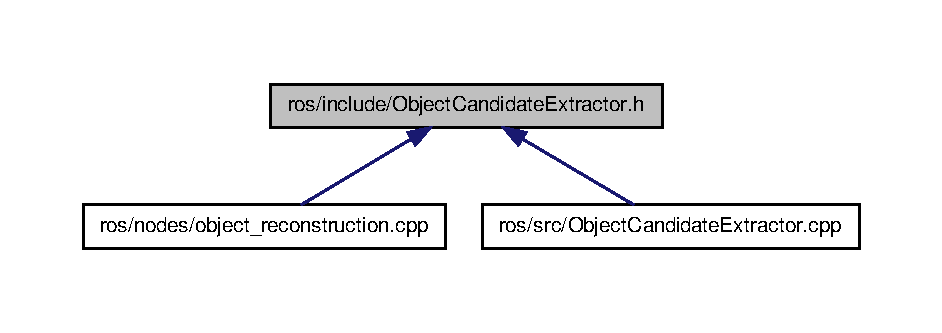
\includegraphics[width=350pt]{_object_candidate_extractor_8h__dep__incl}
\end{center}
\end{figure}
\subsection*{\-Classes}
\begin{DoxyCompactItemize}
\item 
class \hyperlink{class_object_candidate_extractor}{\-Object\-Candidate\-Extractor}
\begin{DoxyCompactList}\small\item\em \-This class is responsible for finding groups of points in a point cloud which could represent real world objects. \end{DoxyCompactList}\end{DoxyCompactItemize}

\hypertarget{_point_cloud_accumulator_8h}{\section{ros/include/\-Point\-Cloud\-Accumulator.h \-File \-Reference}
\label{_point_cloud_accumulator_8h}\index{ros/include/\-Point\-Cloud\-Accumulator.\-h@{ros/include/\-Point\-Cloud\-Accumulator.\-h}}
}
\-Include dependency graph for \-Point\-Cloud\-Accumulator.\-h\-:\nopagebreak
\begin{figure}[H]
\begin{center}
\leavevmode
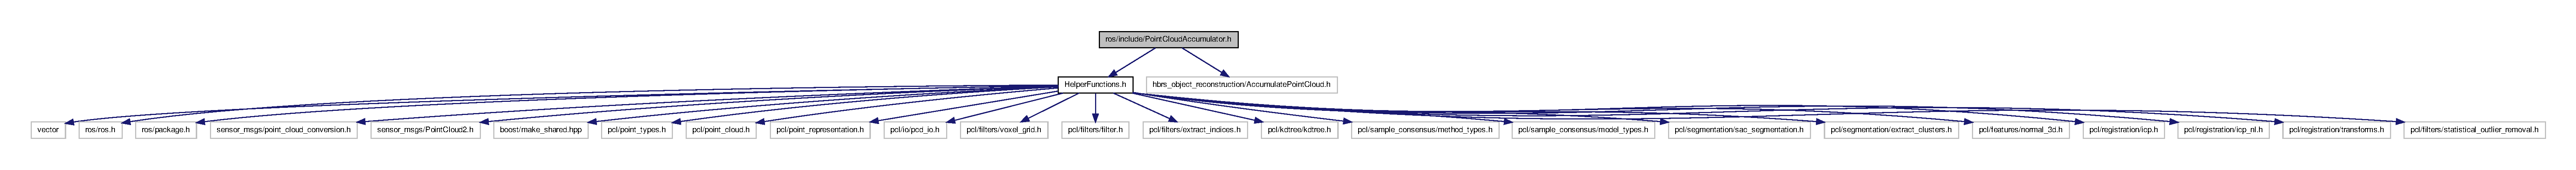
\includegraphics[width=350pt]{_point_cloud_accumulator_8h__incl}
\end{center}
\end{figure}
\-This graph shows which files directly or indirectly include this file\-:\nopagebreak
\begin{figure}[H]
\begin{center}
\leavevmode
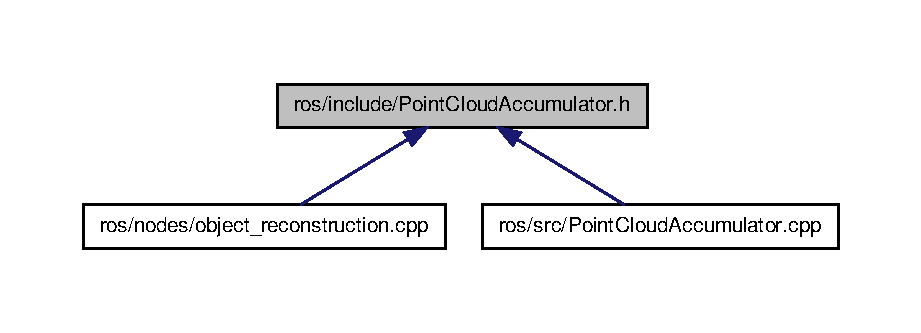
\includegraphics[width=350pt]{_point_cloud_accumulator_8h__dep__incl}
\end{center}
\end{figure}
\subsection*{\-Classes}
\begin{DoxyCompactItemize}
\item 
class \hyperlink{class_point_cloud_accumulator}{\-Point\-Cloud\-Accumulator}
\begin{DoxyCompactList}\small\item\em \-This class takes two point clouds and merges them together. \end{DoxyCompactList}\item 
class \hyperlink{class_my_point_representation}{\-My\-Point\-Representation}
\begin{DoxyCompactList}\small\item\em \-A new representation of \-Point\-Clouds to include \{\-X,\-Y,\-Z,\-Curvature\} information. \end{DoxyCompactList}\end{DoxyCompactItemize}

\hypertarget{object__reconstruction_8cpp}{\section{ros/nodes/object\-\_\-reconstruction.cpp \-File \-Reference}
\label{object__reconstruction_8cpp}\index{ros/nodes/object\-\_\-reconstruction.\-cpp@{ros/nodes/object\-\_\-reconstruction.\-cpp}}
}
\-Include dependency graph for object\-\_\-reconstruction.\-cpp\-:\nopagebreak
\begin{figure}[H]
\begin{center}
\leavevmode

\includegraphics[width=350pt]{object__reconstruction_8cpp__incl}
\end{center}
\end{figure}
\subsection*{\-Classes}
\begin{DoxyCompactItemize}
\item 
class \hyperlink{classobject__reconstruction__node}{object\-\_\-reconstruction\-\_\-node}
\begin{DoxyCompactList}\small\item\em \-This class is responisble for handeling everything that is related to the object reconstruction. \end{DoxyCompactList}\end{DoxyCompactItemize}
\subsection*{\-Functions}
\begin{DoxyCompactItemize}
\item 
int \hyperlink{object__reconstruction_8cpp_a3c04138a5bfe5d72780bb7e82a18e627}{main} (int argc, char $\ast$$\ast$argv)
\begin{DoxyCompactList}\small\item\em \-This is the main class for the object reconstruction. \-It is responsible for starting the processing and launching the object reconstruction node. \end{DoxyCompactList}\end{DoxyCompactItemize}


\subsection{\-Detailed \-Description}
\begin{DoxyAuthor}{\-Author}
\-Matthew \-S \-Roscoe 
\end{DoxyAuthor}
\begin{DoxyDate}{\-Date}
\-July 30th 2013 
\end{DoxyDate}
\begin{DoxyCopyright}{\-Copyright}
\-G\-N\-U \-Public \-License. 
\end{DoxyCopyright}


\subsection{\-Function \-Documentation}
\hypertarget{object__reconstruction_8cpp_a3c04138a5bfe5d72780bb7e82a18e627}{\index{object\-\_\-reconstruction.\-cpp@{object\-\_\-reconstruction.\-cpp}!main@{main}}
\index{main@{main}!object_reconstruction.cpp@{object\-\_\-reconstruction.\-cpp}}
\subsubsection[{main}]{\setlength{\rightskip}{0pt plus 5cm}int {\bf main} (
\begin{DoxyParamCaption}
\item[{int}]{argc, }
\item[{char $\ast$$\ast$}]{argv}
\end{DoxyParamCaption}
)}}\label{object__reconstruction_8cpp_a3c04138a5bfe5d72780bb7e82a18e627}


\-This is the main class for the object reconstruction. \-It is responsible for starting the processing and launching the object reconstruction node. 


\begin{DoxyParams}{\-Parameters}
{\em argc} & \-The input arguments as a std\-::string \\
\hline
{\em argv} & \-The number of input arguments. \\
\hline
\end{DoxyParams}
\begin{DoxyReturn}{\-Returns}
\-Overall program success status. 
\end{DoxyReturn}
\-Initialize this \-R\-O\-S node.

\-Create an instance of the object reconstruction.

\-Start the \-R\-O\-S processing for this node. 
\hypertarget{_helper_functions_8cpp}{\section{ros/src/\-Helper\-Functions.cpp \-File \-Reference}
\label{_helper_functions_8cpp}\index{ros/src/\-Helper\-Functions.\-cpp@{ros/src/\-Helper\-Functions.\-cpp}}
}
\-Include dependency graph for \-Helper\-Functions.\-cpp\-:\nopagebreak
\begin{figure}[H]
\begin{center}
\leavevmode

\includegraphics[width=350pt]{_helper_functions_8cpp__incl}
\end{center}
\end{figure}

\hypertarget{_object_candidate_extractor_8cpp}{\section{ros/src/\-Object\-Candidate\-Extractor.cpp \-File \-Reference}
\label{_object_candidate_extractor_8cpp}\index{ros/src/\-Object\-Candidate\-Extractor.\-cpp@{ros/src/\-Object\-Candidate\-Extractor.\-cpp}}
}
\-Include dependency graph for \-Object\-Candidate\-Extractor.\-cpp\-:\nopagebreak
\begin{figure}[H]
\begin{center}
\leavevmode
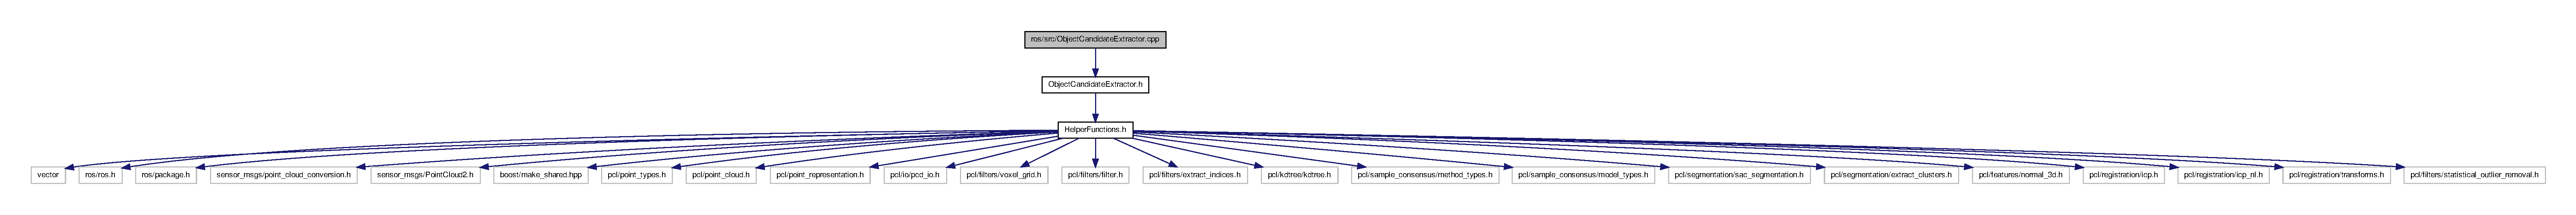
\includegraphics[width=350pt]{_object_candidate_extractor_8cpp__incl}
\end{center}
\end{figure}

\hypertarget{_point_cloud_accumulator_8cpp}{\section{ros/src/\-Point\-Cloud\-Accumulator.cpp \-File \-Reference}
\label{_point_cloud_accumulator_8cpp}\index{ros/src/\-Point\-Cloud\-Accumulator.\-cpp@{ros/src/\-Point\-Cloud\-Accumulator.\-cpp}}
}
\-Include dependency graph for \-Point\-Cloud\-Accumulator.\-cpp\-:\nopagebreak
\begin{figure}[H]
\begin{center}
\leavevmode

\includegraphics[width=350pt]{_point_cloud_accumulator_8cpp__incl}
\end{center}
\end{figure}

\printindex
\end{document}
